\section{Introduction}
% Main goal: Argue for SC, and \xQ. Present \xQ{} and justify decisions. Demonstrate the performance on `realistic simulations'.

Thanks to exciting new advances in artificial intelligence and machine learning, unmanned autonomous physical systems (APS) are poised to tackle complex decision making problems for high-consequence applications, such as wilderness search and rescue, air and ground transportation, national defense, agriculture, manufacturing, and remote science and space exploration. 
Unlike low-level automation for factory assembly lines, vehicle cruise control, building thermostats, etc., APS are expected to be self-sufficient and make self-guided decisions about complex open-ended problems delegated by users/stakeholders. APS that are taskable -- able to translate high-level commands into suitable processes for sensing, learning, reasoning, communicating, and acting under uncertainty -- must also be cognizant and knowledge-rich -- capable of introspectively reasoning about the capabilities and limitations of their own processes, anticipating possible failures, and able to recognize when the are operating incorrectly to adapt accordingly. To ensure long-term robustness and resilience for minimally supervised operations, APS behaviors must be predictable, understandable, and explainable to human users/stakeholders, who in many cases can also provide collaborative high-level assistance or supervisory directives in difficult situations. \nisar{cite DOD studies, etc..}

This work is motivated by the need to develop new computational strategies for cognizance and transparent meta-reasoning to assess when an APS reaches its \emph{competency boundaries}. If computed and communicated correctly, such assessments can provide users with clearer predictions of APS behavior and understanding of actual APS capabilities. This can not only allow APS to take initiatives to stay within its competency boundary in untested/untestable situations, but also provide users/stakeholders with assurances that allow them to properly calibrate trust in (and hence make proper use of) intelligent APS \cite{Israelsen-ACM-2018}. 

These properties are especially important for high-consequence settings in which APS tend to rely heavily on non-deterministic algorithms and approximations for decision-making under uncertainty, in order to efficiently make inferences with imperfect models and learn from limited data. 
%From self-driving cars and unmanned aircraft on Earth to planetary rovers in space \cite{}, and from networked smart devices in the home to smart building systems \cite{}, such APS are now becoming a pervasive part of everyday reality. 
%Crucially, these systems require interaction among several different algorithmic components to support intelligent APS capabilities (for sensing, perception, planning, control, communication, etc.). 
%Algorithms for these capabilities are often studied in isolation, but not together... 
%\nisar{but not much work has been done in terms of holistically looking at APS operating under uncertainty -- expand on this in background...} 
Whereas most relevant work on algorithmic introspection and meta-reasoning to date %for intelligent and learning agents 
has focused on outcome-based analyses for intelligent/learning agents with narrowly defined capabilities and virtually no physical computing/execution limitations, machine self-confidence places a stronger emphasis on process-based analysis for embodied systems (i.e. an engineered sum of several interconnected algorithmic and physical parts). Such systems must operate in more open-ended task settings in physical environments (with significant computing limits due to constrained platform size, weight, and power) where the interpretation of `favorable/unfavorable' outcomes can shift in subtle but significant (and sometimes surprising) ways as a function of APS design and task context. 

In this paper, we present and build on a recently developed algorithmic framework for computing and evaluating self-assessments in APS that leads to shorthand metrics of \emph{machine self-confidence}. Self-confidence is defined as an APS' perceived ability to achieve assigned goals after accounting for uncertainties in its knowledge of the world, its own state, and its own reasoning and execution abilities \cite{Aitken2016-cv, Aitken2016-fb, Sweet2016-tz}. 
Algorithmic computation of self-confidence is strongly linked to model-based assessments of probabilities pertaining to task outcomes and completion -- but crucially goes further to provide insight into how well an APS's processes for decision-making, learning, perception, etc. are matched to intended tasks \cite{Hutchins2015-if}. 
We argue that the short-hand insight provided by self-confidence assessments can serve as a transparent and decomposable/traceable feedback signal to anticipate degraded, nominal, or enhanced APS performance -- %adapt autonomous behavior, 
and thereby can be used to calibrate user trust in APS operating in uncertain dynamic task settings. 

...So what are we doing in this paper exactly: provide a brief overview of our factorized machine self-confidence (FaMSeC) framework in the context of autonomous decision-making, and discuss key principles/ideas...then focus on idea of solver quality for decision making under uncertainty in the context of MDPs -- which are the foundation of things like reinforcement learning, etc. and are widely used as framework for robotics, etc...in doing this, we set up an example concrete grounding problem inspired by our work with unmanned vehicles...then show some preliminary computational results and discuss ongoing/future work...within the scope of FAT* `topics of interest' we fall under the \emph{Transparency} branch. Specifically `Interpretability of ML models', and `Generation of explanations' (although probably more interpretability according to most people's definitions).

\nisar{very important: need a statement of contributions -- why should this audience care about this work? what is the intellectual contribution? (would be good to see other papers from previous year's proceedings to see examples)...}
within the scope of the FAT* tracks I believe that we align with:
\begin{enumerate}
    \item Statistics, Machine Learning, and Data Mining
    \item HCI, and Information Visualiation
    \item \ldots possibly something along the lines of empirical studies, as that is what we intend to do
\end{enumerate}


%\nisar{can probably borrow text from Matt's RSS paper and Nick's InfoTech paper to help establish the context and motivation for this work...to argue for need for assurances and self-confidence, need to first establish that autonomous systems/robots are here and rely heavily on ML techniques as well as decision-making algorithms to operate under uncertainty...difficult to ensure transparency because same inputs/operating conditions may lead to different behaviors, which in turn affects user trust...lots of work lately on trust in autonomous systems (cite some refs), which relates very closely to question of how to establish transparency and explainability and predictability, etc. for ML systems...key difference is that autonomous systems are to a large extent expected to be self-directed and self-sufficient decision makers -- though, in reality, they must operate within a delegated scope of action and competency (cite Johnson's `Seven Deadly Myths of Autonomous Systems') ... thus the transparency/explainability question in this case is: how does a system know its own limits and convey this to a user/stakeholder? Or, equivalently: how can an autonomous system justify it's ability to accomplish a task? note: they key insight we bring to the table here is that the question of introspection and communication of a machine's own limits is itself a complex problem of meta-reasoning that requires its own set of AI/learning approaches to tackle...leads to idea of algorithmic self-confidence as an assurance...  }

% We can choose `archival' or `non-archival'. I think we probably want to do archival, since this is a promising `home' for our research anyway.

% \subsection{Proposed outline:}

% \begin{itemize}
%     \item Motivation---why MDPs, why meta-analysis, why self-confidence? \nisar{should add in some background about autonomous systems concepts that are relevant for this audience to pick up key ideas...}
%     \item Related work---quickly review some related work in the area \nisar{what other ideas specifically should be mentioned?}
%     \item Approach---desiderata, Hellinger distance, etc
%     \item Results/Discussion---Illustrative example, and theoretical example
%     \item Conclusions/Future Work---restate purpose of SC, and particularly \xQ. Discuss continuing efforts to quantify effects with human-involved experiments. Further development of \xH, \xI, and \xM.
% \end{itemize}

\subsection{Related Work}
    Discuss related work such as

    WHY DO WE USE MDPS? THEY ARE A GOOD PLACE TO START FROM, AND ARE CONNECTED TO MANY OTHER LEARNING APPROACHES (REINFORCEMENT, INVERSE REINFORCEMENT, \ldots)

    Reinforcement learning is finding a policy when transitions, and states are unknown. Basically learn policy and model simultaneously.

    inverse RL is learning a reward function by observing a policy.

\subsection{Factorized Machine Self-Confidence}
    \begin{figure*}[tbp]
        \centering
        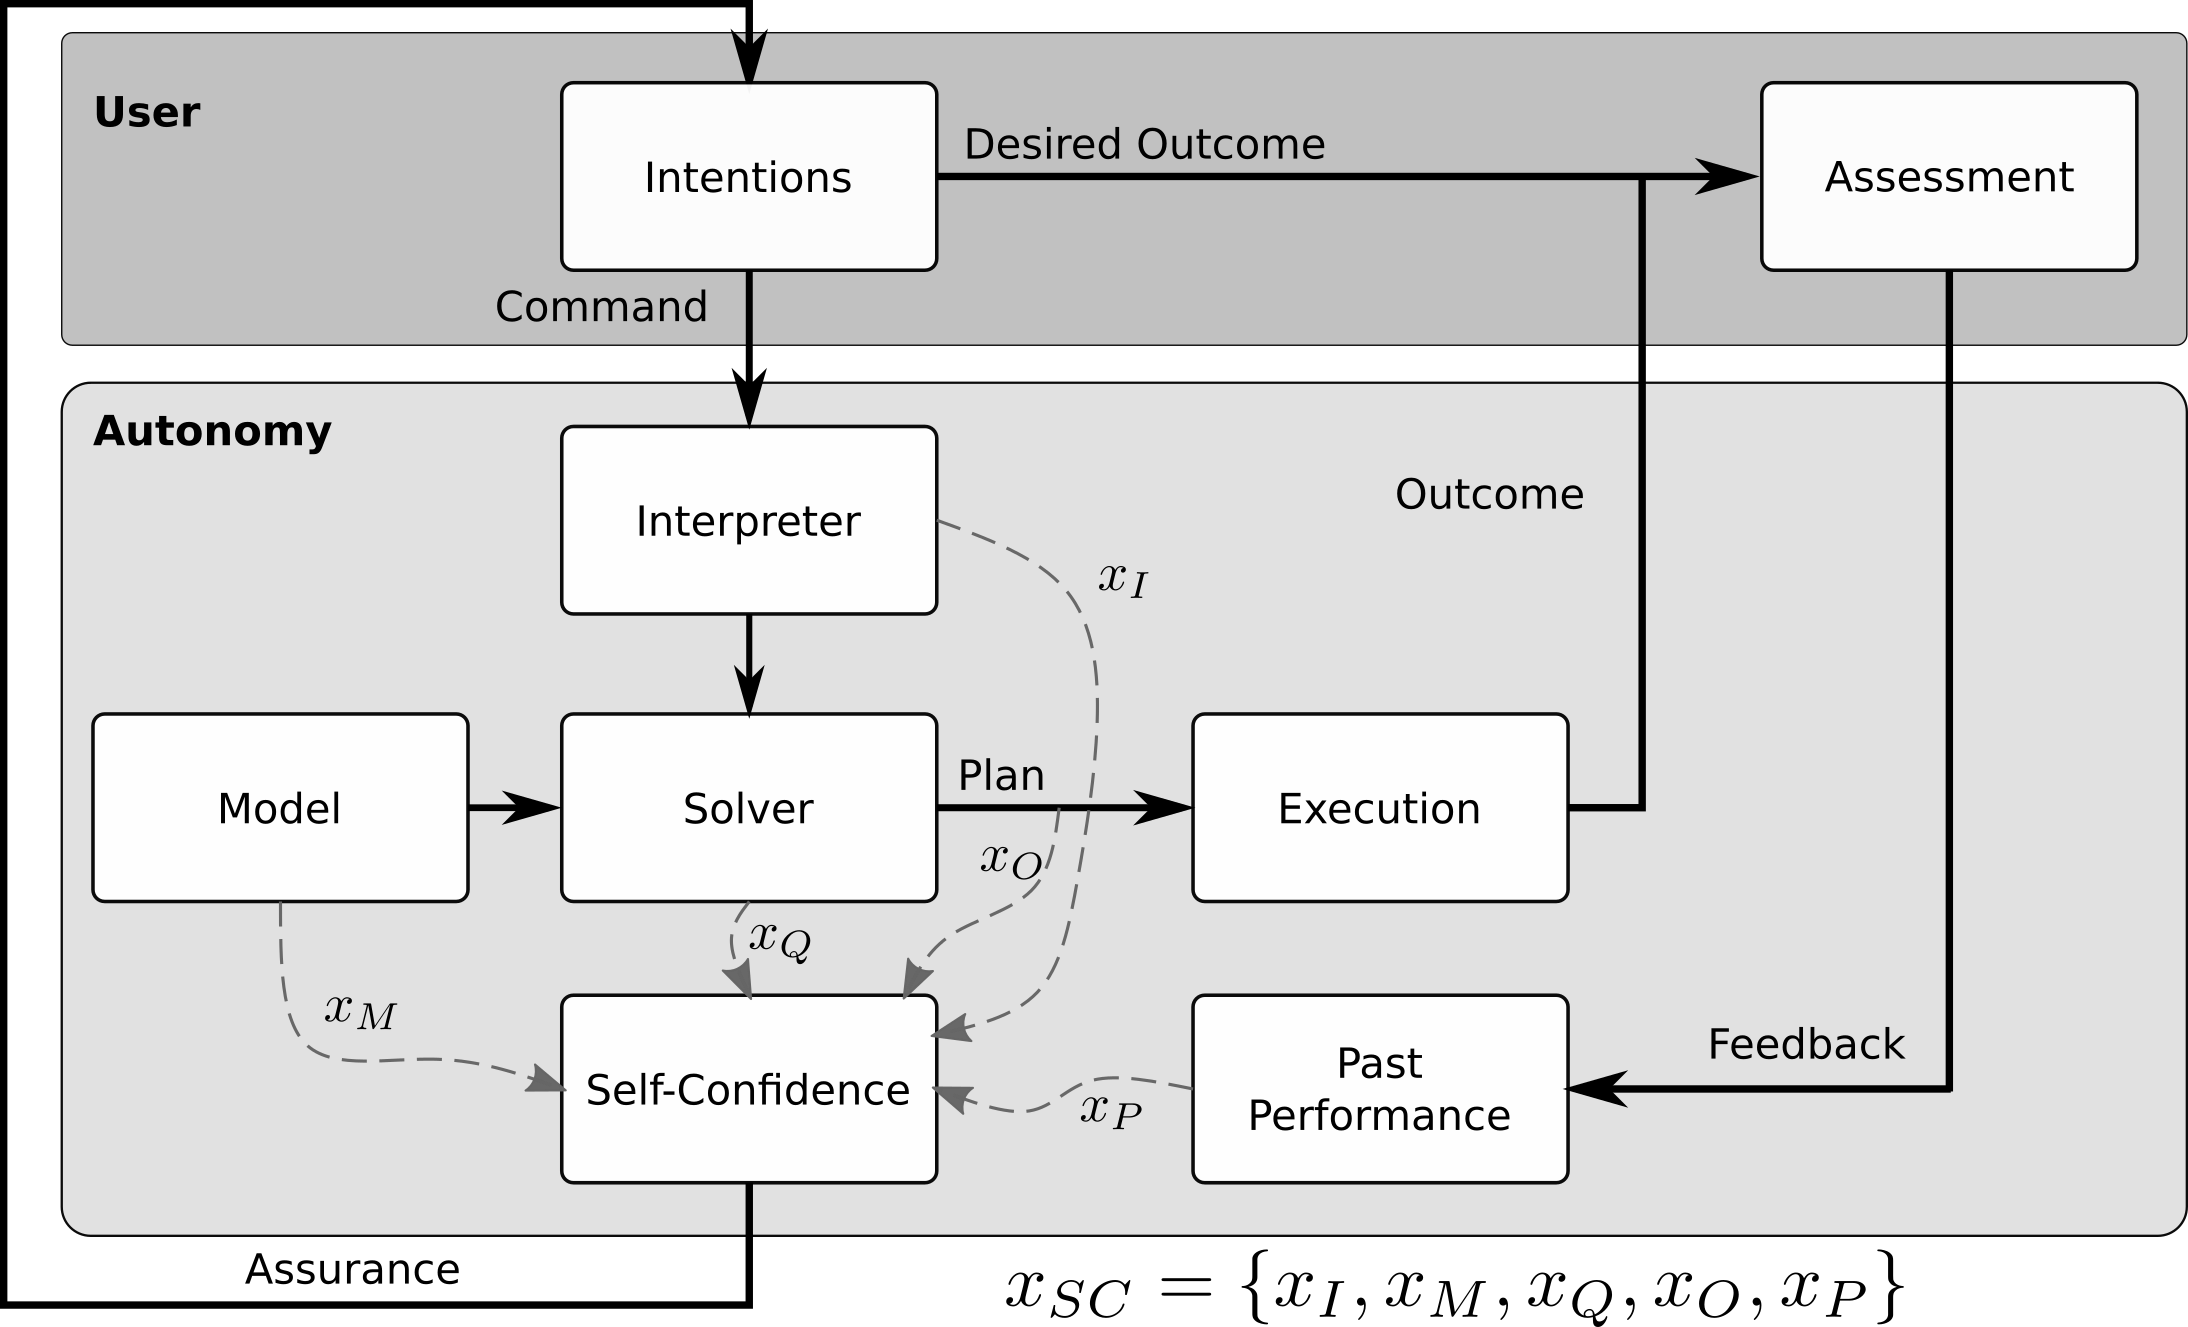
\includegraphics[width=0.55\linewidth]{Figures/FaMSeC.png}
        \caption{Factorized Machine Self-Confidence (FaMSeC)}
        \label{fig:famsec}
    \end{figure*}

    Several definitions of machine self-confidence have been proposed in recent works. Much of this work is reviewed in \cite{Israelsen2017-ym}, where self-confidence is identified as an explicit assurance in a human-autonomy trust relationship. According to \cite{Sweet2016-tz} the four views on self-confidence are the \textit{anthropomorphic view}, the \textit{uncertainty view}, the \textit{experiential view}, and the \textit{stability view}. The anthropomorphic view defines self-confidence to be similar to how humans express self-confidence, while the experiential view expresses self-confidence based on past experience. The uncertainty view simply defines self-confidence to be the probability of success or failure, and the stability view defines self-confidence to be the sensitivity of the probability of success to uncertainty. All of these views seem to reflect different parts of a more general concept: understanding an autonomy's ability to do a specific task. This leads to our definition of self-confidence: \textbf{An agent's perceived ability to achieve assigned goals (within a defined region of autonomous behavior) after accounting for (1) uncertainties in its knowledge of the world, (2) uncertainties of its own state, and (3) uncertainties about its reasoning process and execution abilities.}

    ...\nisar{edit:} The formal definition of self-confidence we use is from \cite{Aitken2016-cv}, wherein five factors that compose self confidence are defined. Figure \ref{fig:famsec} highlights at what point in a autonomous system's logic each of the factors originate. They are: \nisar{can add some more detail from proposals...}

        \begin{itemize}
            \item [\xH{}:] \textbf{Past Performance}---how well has autonomy done in similar circumstances?
            \item [\xI{}:] \textbf{Command Interpretation}---are autonomy and user `on the same page'?
            \item [\xM{}:] \textbf{Model Validity}---How well does autonomy's model reflect reality?
            \item [\xP{}:] \textbf{Predicted Outcome Assessment}---How favorable is the distribution of predicted outcomes?
            \item [\xQ{}:] \textbf{Solver Quality}---How well can the solver use the model to generate policies/plans?
        \end{itemize}

    Self-confidence \xSC{} is a composite assurance that stems from some combination of these five factors. \xP{} has been previously defined in \cite{Aitken2016-cv}, but has not yet been evaluated as an effective assurance as per the guidelines laid out in the work on assurances. Herein \xQ{} is investigated.

\subsection{Solver Quality (\xQ)} \label{sec:SQ}
    The main aim of \xQ{} is to indicate how a solver \solve{} will perform on a given (possibly un-encountered) task \task{}. Formally, the desiderata are:

    \begin{enumerate}[label=\textbf{D\arabic*}]
        \item reflect competence of solver \solve{} for task \task{} \label{itm:d1}
        \item enable comparison across solver classes \label{itm:d2}
        \item extend to unseen tasks \label{itm:d3}
    \end{enumerate}
    
    Evaluating the `quality' of something implies some kind of comparison is taking place. In this setting the desired comparison is between a `candidate solver' \solve{} and some reference solver. Ideally, the candidate solver could be compared to the exact solution, but there are three main challenges:

    \begin{enumerate}[label=\textbf{C\arabic*}]
        \item It is unclear how policies should be compared \label{itm:l1}
        \item Exact solutions to most practical problems are infeasible due to large state-spaces \label{itm:l2}
        \item Even if \ref{itm:l2} weren't an issue, it is generally impossible to evaluate the performance of any solver on \emph{all} possible problems \label{itm:l3}
    \end{enumerate}

    \subsubsection{Addressing \ref{itm:l1}} \label{sec:compare_policies}
        Solvers of all classes are similar in that they operate on a specified problem, and have defined solver parameters that govern their behavior, in order to produce a policy $\pi$ that is a mapping from states to actions. A few possibilities for comparing policies include:
    
        \begin{enumerate}
            \item Compare utilities at each state \label{itm:i1}
            \begin{itemize}
                \item Merits: Evaluates whether states are assigned equal utility across solvers. Theoretically state utilities should be independent of the solver. Addresses \ref{itm:d1}
                \item Demerits: Does not apply to solvers that represent different amounts of the state-action space (i.e. exact versus approximate solvers), or to solvers that may represent the state-action space differently (i.e. meta-solvers). This approach does not satisfy \ref{itm:d2}.
            \end{itemize} 
            \item Compare `coverage' of the policy (here coverage refers to the proportion of the state space considered by the solver) \label{itm:i2}
            \begin{itemize}
                \item Merits: Evaluates how `thorough' the policy is, in concert with \ref{itm:i1} could address \ref{itm:d1}
                \item Demerits: Does not meet \ref{itm:d2} because not all policies will have the same coverage by design. Also high coverage does not imply a `good' solution
            \end{itemize}
            \item Compare the reward distribution of given policies \label{itm:i3}
            \begin{itemize}
                \item Merits: Meets \ref{itm:d1}, also able to satisfy \ref{itm:d2} as reward distributions can be simulated from any policy
                \item Demerits: Expensive to calculate the reward distribution via many simulations
            \end{itemize}
        \end{enumerate}

        Of the possibilities listed above, item \ref{itm:i3} will be used because only it is able to satisfy \ref{itm:d1} and \ref{itm:d2}.

    \subsubsection{Addressing \ref{itm:l2}, and \ref{itm:l3}} \label{sec:practicality}
        In order to address \ref{itm:l2} a `trusted solver' \solvestar{} could be introduced as the reference to which the candidate solver \solve{} can be compared. This solver need not be exact (but could be). Ultimately, \solvestar{} is only required to be a reference of some kind; it may be optimal, or it may be abysmal. In fact given a space of all possible unseen tasks of class $\text{some task class notation}$, \solvestar{} will likely be abysmal for some of them.

        Still according to \ref{itm:l3} it is impractical, or impossible, to make an exact solution for all tasks $\text{task class notation}$. Literature on `Empirical Hardness Models' (EHMs) lends some direction for confronting this challenge. In their work \cite{Leyton-Brown2009-yr,Hutter2009-og} introduced EHMs in order to predict the empirical runtime performance of an algorithm on a problem with given features \brett{add some more detail about the approach, I think they used SAT*}. Applying similar logic in this domain, it should be possible to learn a surrogate model \surrogate{} that predicts the reward distribution \rwdstarapprox{} of the trusted solver \solvestar{} for a given task \task. In this way it is possible to estimate the performance of \solvestar{} on problems to which it has never been applied.
